\documentclass[10pt]{article}
\usepackage[utf8]{inputenc}
\usepackage[T1]{fontenc}
\usepackage{amsmath}
\usepackage{amsfonts}
\usepackage{amssymb}
\usepackage[version=4]{mhchem}
\usepackage{stmaryrd}
\usepackage{graphicx}
\usepackage[export]{adjustbox}
\graphicspath{ {./images/} }

\title{SOLUTIONS FOR EXTRA ADMISSIONS TEST IN MATHEMATICS, COMPUTER SCIENCE AND JOINT SCHOOLS NOVEMBER 2023 }

\author{}
\date{}


\begin{document}
\maketitle
A Each of the given polynomials is of the form $y=x^{3}-3 x^{2}+k x$. The first derivative is $3 x^{2}-6 x+k$, and the second derivative is $6 x-6$. So if there is a point with zero derivative, then it will either be a local maximum or a local minimum, unless $x=1$. At $x=1$ the first derivative is $k-3$, which is only zero if $k=3$.

The answer is (c)

B Note that $\sqrt[10]{10^{11}}$ is $10^{11 / 10}$, so $\log _{10}\left(\sqrt[10]{10^{11}}\right)=\frac{11}{10}$. This is less than $\frac{11}{9}$.

To compare $\sqrt{\frac{3}{2}}$ with $\frac{11}{10}$, compare their squares; compare $\frac{3}{2}$ with $\frac{121}{100}$. The former is $\frac{150}{100}$ which is larger than $\frac{121}{100}$.

Now note that $\sqrt{3} \cos \left(44^{\circ}\right)$ is slightly larger than $\sqrt{3} \cos \left(45^{\circ}\right)$ which is $\sqrt{\frac{3}{2}}$.

Finally note that $\pi>3$ so $\frac{\pi}{2}>\frac{3}{2}>\frac{11}{10}$.

So the smallest of the numbers is $\frac{11}{10}$.

The answer is (a)

C The required sum is the sum of all cubes up to $20^{3}$ minus the sum of the even cubes up to $20^{3}$.

$$
\begin{aligned}
1^{3}+3^{3}+5^{3}+7^{3}+\cdots+19^{3} & =\left(1^{3}+2^{3}+3^{3}+4^{3}+\cdots+20^{3}\right)-\left(2^{3}+4^{3}+6^{3}+\cdots+20^{3}\right) \\
& =\left(1^{3}+2^{3}+3^{3}+4^{3}+\cdots+20^{3}\right)-2^{3}\left(1^{3}+2^{3}+3^{3}+\cdots+10^{3}\right) \\
& =\frac{20^{2} \times 21^{2}}{4}-8 \times \frac{10^{2} \times 11^{2}}{4} \\
& =10^{2} \times\left(21^{2}-2 \times 11^{2}\right) \\
& =10^{2} \times(441-2 \times 121) \\
& =19,900
\end{aligned}
$$

\section*{The answer is (b)}
D The numbers $x$ and $y$ are each either odd or even, so the squares $x^{2}$ and $y^{2}$ are each either multiples of 4 or one more than a multiple of 4 . There are four cases to check, and after checking each, we find that the expression on the left-hand side could be a multiple of 4 (if $x$ and $y$ are both even, or both odd), or could be one more than a multiple of 4 (if $x$ is odd and $y$ is even), or could be three more than a multiple of 4 (if $x$ is even and $y$ is odd). The number on the right-hand side is two more than a multiple of 4 . So there are no solutions.

The answer is (a)

E Starting with 1, there are nine one-digit numbers. Then from 11 to 99 there are 90 two-digit numbers, then there are 900 three-digit numbers, and so on. So the required sum is (grouping terms by the number of digits of $n$ ) equal to

$$
9 \times 20^{-1}+90 \times 20^{-2}+900 \times 20^{-3}+\ldots
$$

which is a geometric series with first term $\frac{9}{20}$, common ratio $\frac{1}{2}$ and sum to infinity equal to $\frac{9}{10}$. The answer is (c)

F If $a=c$ and $b=d$ then the expression we're given for $f\left(\left(\begin{array}{l}a \\ b\end{array}\right),\left(\begin{array}{l}c \\ d\end{array}\right)\right)$ becomes $\left(\begin{array}{c}a^{2}+b^{2} \\ 2 a b+b^{2}\end{array}\right)$.

We're looking for whole numbers (positive or negative or zero) for $a$ and $b$ such that $a^{2}+b^{2}=2$ and $2 a b+2 b^{2}=0$. From the second equation we conclude that $b=0$ or $a+b=0$. If $b=0$ then $a^{2}=2$ but there are no whole numbers that square to 2 . If $a+b=0$ then we can eliminate $b$ from the first equation and conclude that $a= \pm 1$. We should check that $\left(\begin{array}{c}1 \\ -1\end{array}\right)$ and $\left(\begin{array}{c}-1 \\ 1\end{array}\right)$ both work.

The answer is (c)

G The triangular numbers described in the question as the sum of the first $k$ positive integers for some $k \geq 1$ have the form $\frac{1}{2} k(k+1)$, if we sum the arithmetic series.

Let's write $N=x+y$. Then $0<y \leq N$ and $f=\frac{1}{2} N(N+1)+y$. In words, first we choose a triangular number and then we add some positive quantity $y$. The number $y$ can never be quite large enough to make the "next" triangular number because the difference between $\frac{1}{2} N(N+1)$ and $\frac{1}{2}(N+1)(N+2)$ is $N+1$. But $f$ can take all other values.

The answer is (e)

H We're told that $2 x^{4}-3 x^{3}-5 x^{2}+2 x+2=m x$ has exactly four real solutions $x_{1}, x_{2}, x_{3}, x_{4}$. Moving the $m x$ to the other side of the equation, the Factor Theorem implies that the resulting polynomial factorises like this;

$$
2 x^{4}-3 x^{3}-5 x^{2}+(2-m) x+2=2\left(x-x_{1}\right)\left(x-x_{2}\right)\left(x-x_{3}\right)\left(x-x_{4}\right),
$$

where we have been careful to include the factor of 2 in order to match the leading coefficient of $x$. Now subsitute $x=0$ in both sides of the equation for the result that $2=2 x_{1} x_{2} x_{3} x_{4}$.

The answer is (b)

I The equations describe grid of parallel lines, with the line $y=1-10 x$ crossing opposite corners and the midpoint of the grid, but no other grid points.

\begin{center}
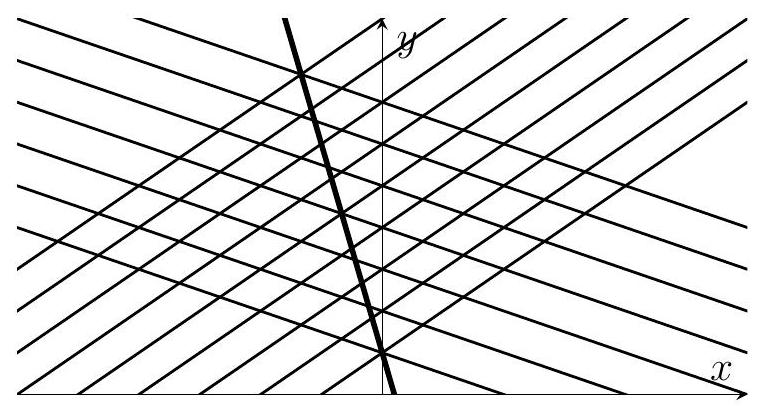
\includegraphics[max width=\textwidth]{2024_03_31_e665606340d23fab60a7g-2}
\end{center}

There would normally be 16 points where the line $y=1-10 x$ crosses 16 given lines, but at three grid points the line $y=1-10 x$ crosses two of the given lines "simultaneously". There are only 13 distinct points where the line $y=1-10 x$ crosses one or more of the other lines.

The answer is (b)

$\mathbf{J}$ The equation rearranges to

$$
x^{4}+4 x^{3} y+6 x^{2} y^{2}+4 x y^{3}+y^{4}=x^{2}
$$

If we recognise the left-hand side as $(x+y)^{4}$ then we can simplify this down to $(x+y)^{4}=x^{2}$. Now if $x$ is positive then $(x+y)^{2}=x$ and so $y=-x \pm \sqrt{x}$. Since $x$ grows faster than $\sqrt{x}$, the value of $y$ is eventually negative for both of these solutions (once $x>1$ ). Only one of the graphs behaves like this.

The answer is (d)


\end{document}